\chapter{Giới thiệu hệ thống}\label{chap1}
Trước khi đi sâu về thiết kế kiến trúc của hệ thống quản lý quán ăn và các dịch vụ liên quan, chương này sẽ trình bày các chức năng chính của hệ thống theo thiết kế cũng như là đi qua luồng nghiệp vụ của một số tính năng cụ thể.
\section*{Các chức năng chính}\label{sec:main-functions}
Mô hình quản lý quán ăn được phát triển trong khóa luận này sẽ tập trung vào các chức năng chính giúp nhà hàng, quán ăn quản lý thực đơn, khách và bàn, v.v.
Từ các chức năng chính như quản lý thực đơn sẽ có các chức năng nhỏ hơn bổ trợ được gọi là các tính năng phụ.
Ví dụ như đối với chức năng quản lý bàn, ngoài các chức năng chính như tạo bàn mới, xóa bàn, thay đổi trạng thái của bàn, v.v., các nhánh chức năng phụ còn bao gồm các chức năng như ghép bàn, phân bàn cho những người đặt bàn trước, v.v.
Danh sách các chức năng chính của hệ thống quản lý quán ăn được mô tả tại Hình~\ref{fig:landing-page-use-case} và Hình~\ref{fig:admin-page-use-case} bao gồm đặt bàn trực tuyến, gọi món thông qua việc quét mã QR, thanh toán hóa đơn, v.v.

\begin{figure}[H]
	\centering
	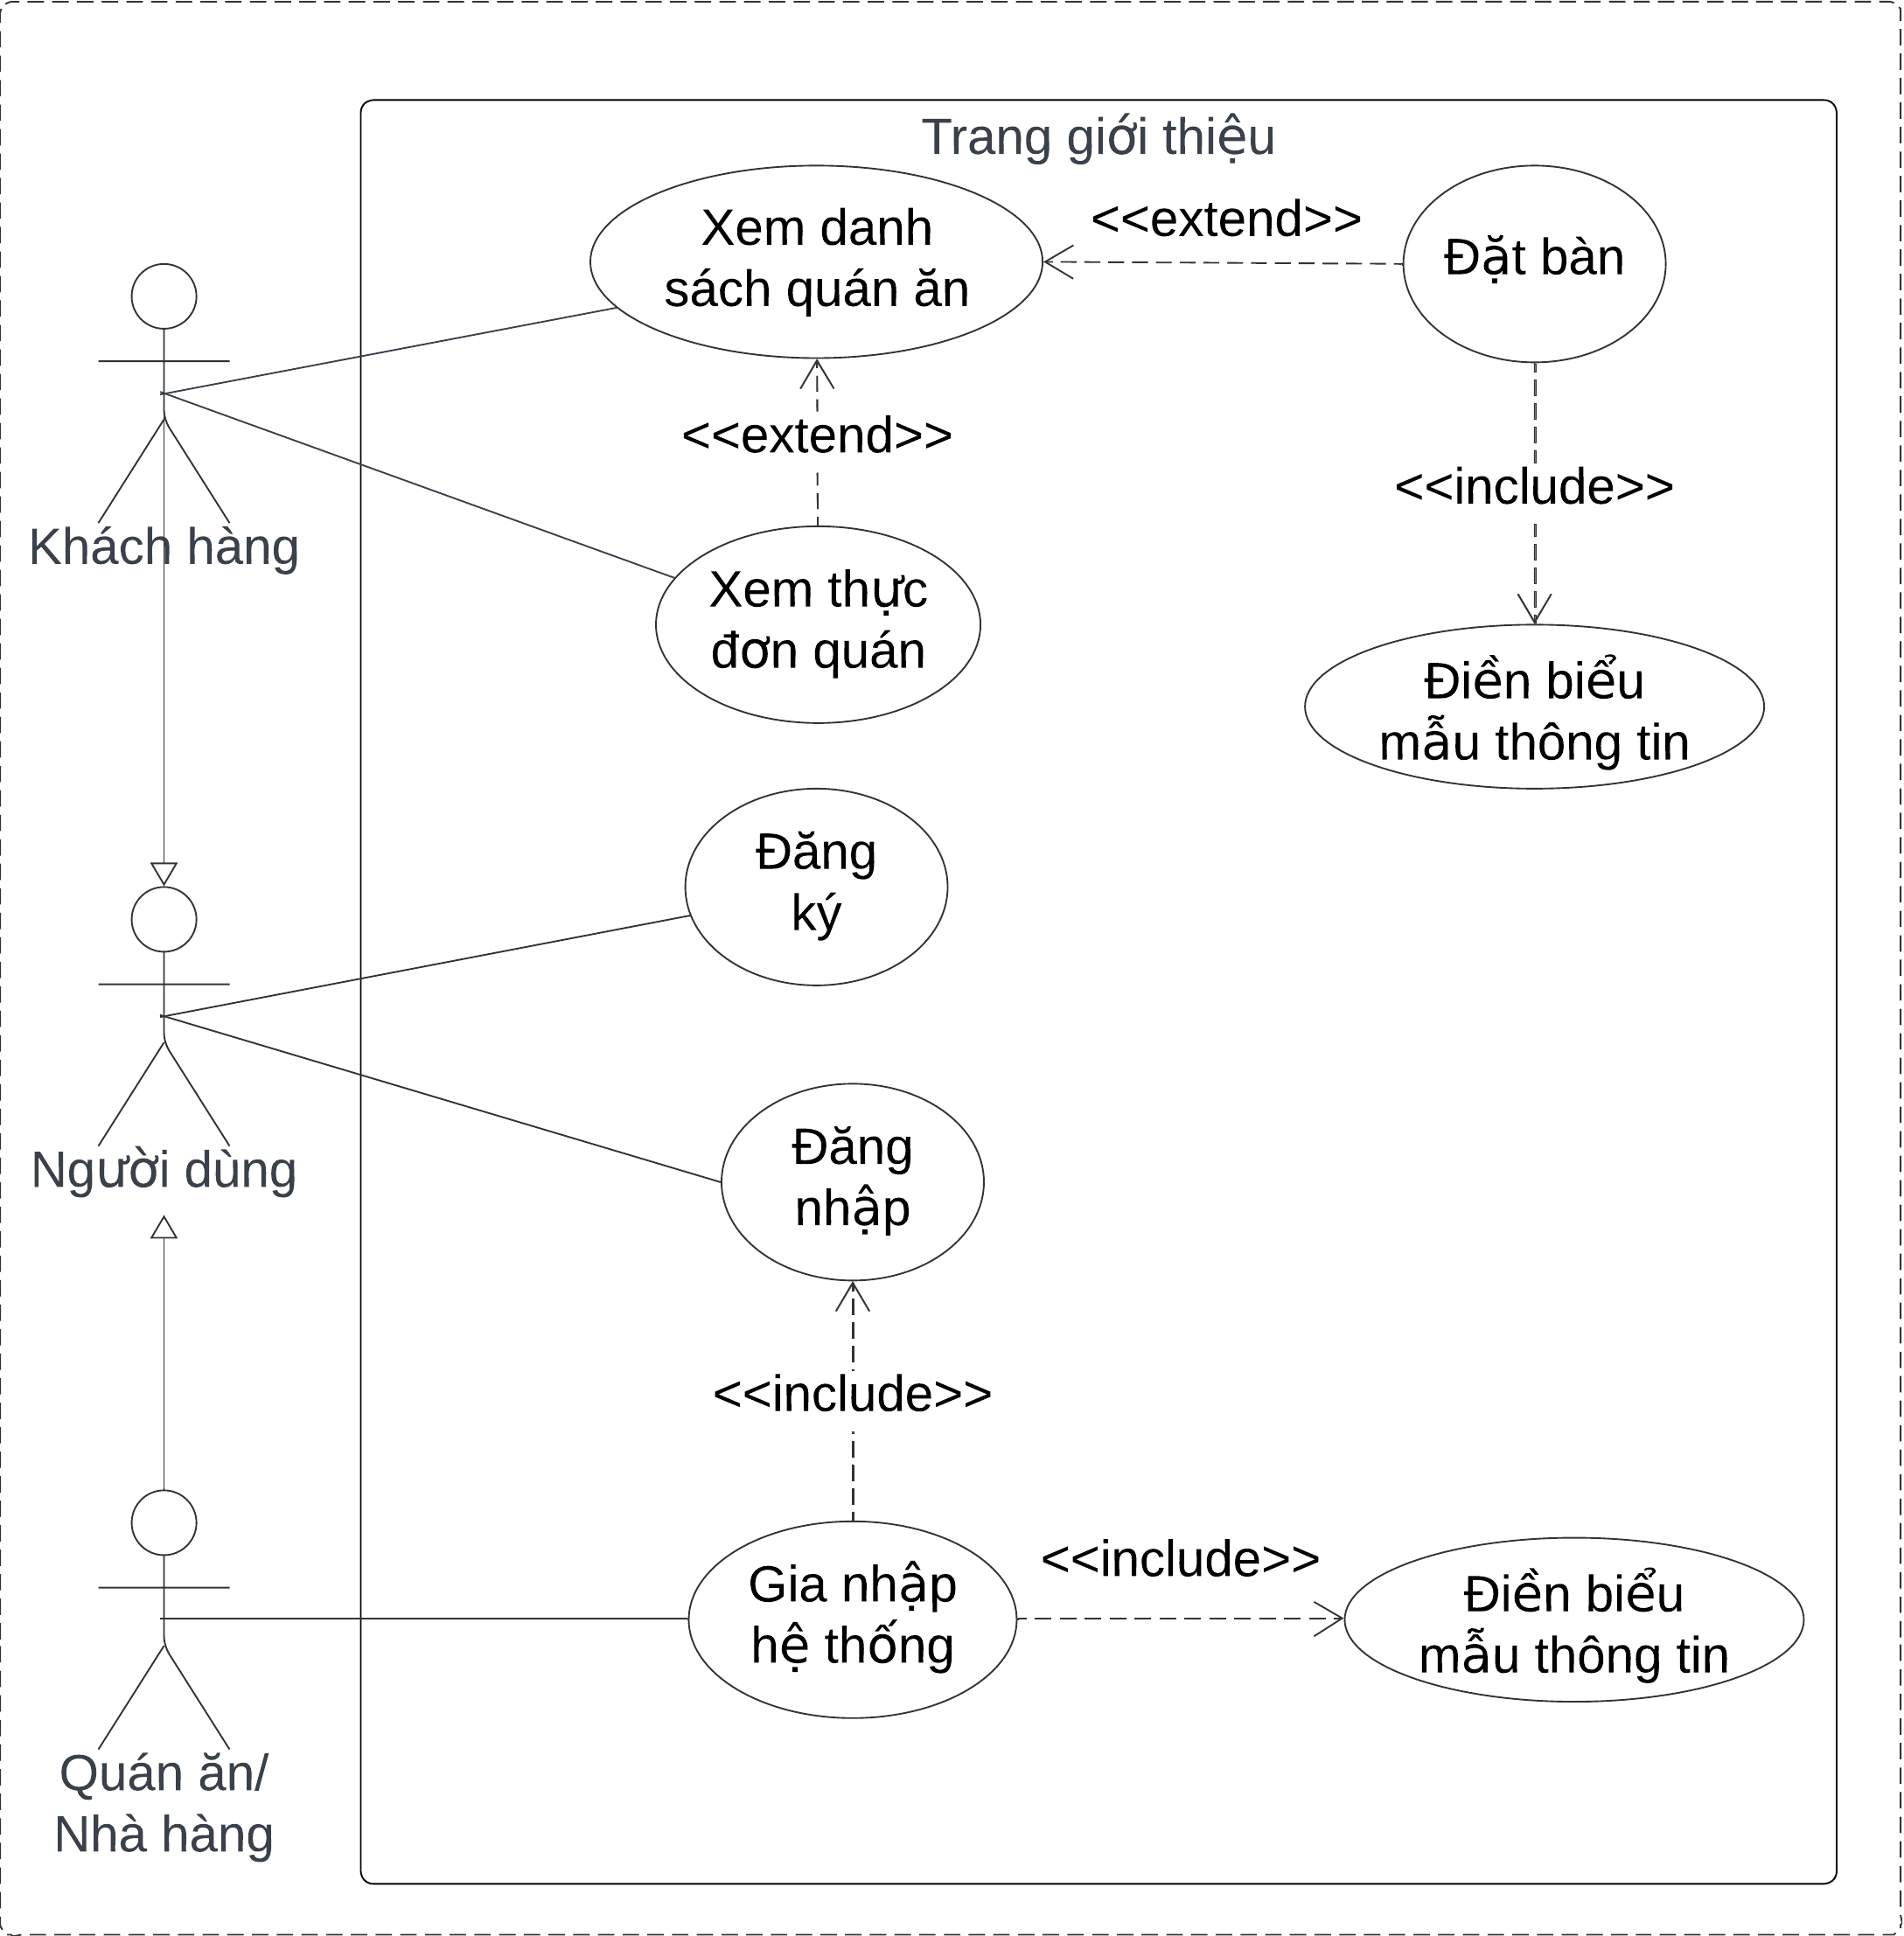
\includegraphics[width=\textwidth]{images/hChip/main-flow/landing-page-use-case-diagram.png}
	\caption{Biểu đồ ca sử dụng cho trang giới thiệu \tcode{landing-page}}
	\label{fig:landing-page-use-case}
\end{figure}

\begin{figure}[H]
	\centering
	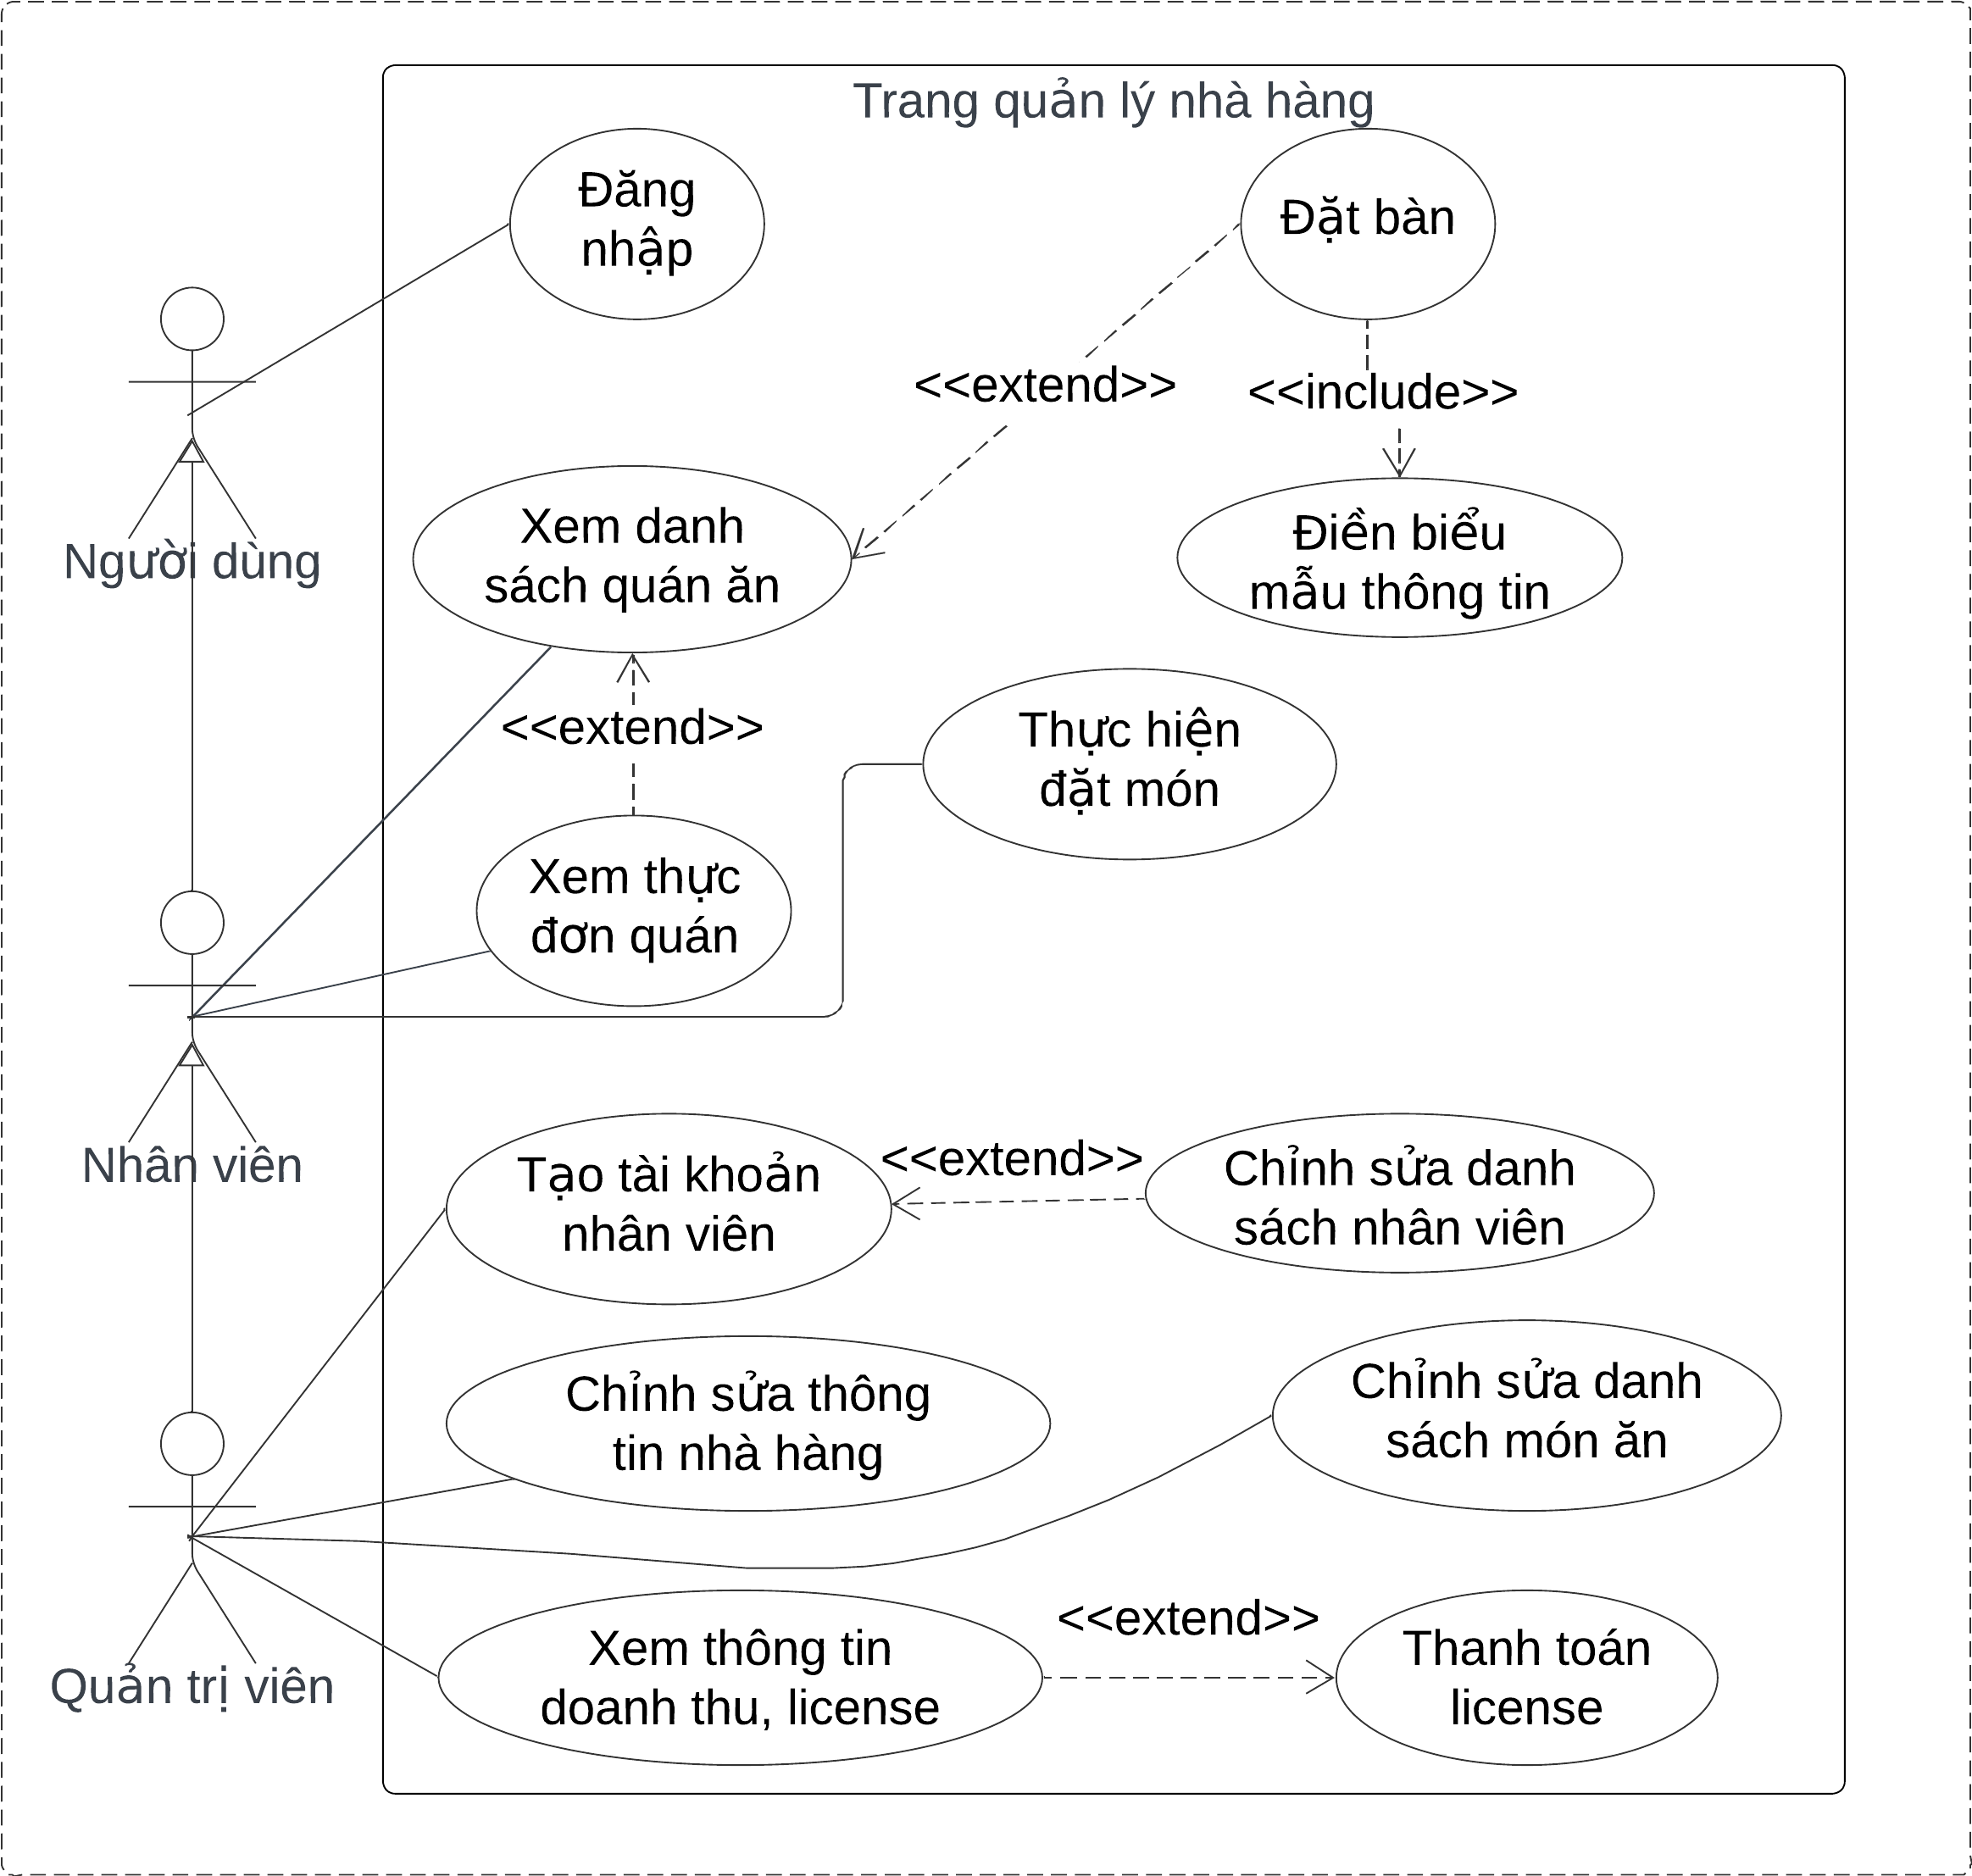
\includegraphics[width=\textwidth]{images/hChip/main-flow/admin-page-use-case-diagram.png}
	\caption{Biểu đồ ca sử dụng cho trang quản lý nhà hàng \tcode{admin-page}}
	\label{fig:admin-page-use-case}
\end{figure}

Luồng đặt bàn trực tuyến và đặt món qua QR sẽ được tập trung thảo luận và mô tả xuyên suốt các chương về sau.
Chương này sẽ tập trung mô tả qua các tác nhân tham gia vào hệ thống và một luồng nghiệp vụ tổng quan giữa các bên tham gia.
Mô tả kỹ thuật các lời gọi API cũng như là các tương tác giữa các vi dịch vụ với nhau sẽ được mô tả rõ hơn tại Mục~\autoref{sec:user-flow-examples}

\subsection*{Luồng đặt bàn trực tuyến}\label{sec:reservation-flow}
Luồng người dùng đặt bàn có thể được tương tác bởi cả người dùng đã đăng ký đăng nhập cũng như là người dùng vãng lai của hệ thống.
Khách hàng có thể sử dụng chức năng đặt bàn tại trang giới thiệu \textit{landing-page} hoặc là trang giới thiệu \textit{customer-page} của nhà hàng, quán ăn đã gia nhập vào nền tảng chung.

\begin{table}[ht]
\caption{Bảng mô tả luồng nghiệp vụ của chức năng đặt bàn trực tuyến}
\label{tab:reservation-flow}
\resizebox{\textwidth}{!}{%
\begin{tabular}{|p{0.05\linewidth}|p{0.2\linewidth}|p{0.35\linewidth}|p{0.4\linewidth}|}
\hline
\textbf{STT} & \multicolumn{1}{c|}{\textbf{Màn hình}}                 & \multicolumn{1}{c|}{\textbf{Hoạt động người dùng}} & \multicolumn{1}{c|}{\textbf{Tương tác hệ thống}} \\ \hline
1            & Trang giới thiệu & Mở ứng dụng/truy cập vào website                   & Hiển thị giao diện trang giới thiệu              \\ \hline
2 & Trang giới thiệu          & Chọn chức năng đặt bàn                            & Chuyển hướng đến trang đặt bàn                                              \\ \hline
3 & Trang đặt bàn             & Nhập các thông tin cần thiết                      & Kiểm tra tính khả dụng của bàn                                              \\ \hline
4 &                           &                                                   & Hiển thị kết quả và trạng thái: bàn trống hoặc không có bàn                 \\ \hline
5 &                           & Nếu có bàn trống: Chọn bàn, xác nhận đặt bàn      &                                                                             \\ \hline
6 &                           &                                                   & Ghi nhận thông tin đặt bàn, gửi thông báo xác nhận, cập nhật trạng thái bàn \\ \hline
7 & Ứng dụng quản lý nhà hàng &                                                   & Hiện thị thông báo đặt bàn mới                                              \\ \hline
8 &                           & Nhân viên nhà hàng phân bàn và xác nhận với khách &                                                                             \\ \hline
\end{tabular}%
}
\end{table}

Ở bước 8 Bảng~\ref{tab:reservation-flow}, nhân viên xác nhận với khách hàng, điều này có thể được thực hiện thông qua nhân viên gọi điện hoặc gửi email xác nhận thông tin đặt bàn.
Các trường thông tin của khách hàng sẽ được lấy từ thông tin tài khoản nếu khách hàng có đăng nhập vào hệ thống hoặc tại biểu mẫu được nhập khi yêu cầu đặt bàn của khách hàng mới.

\subsection*{Luồng đặt món thông qua quét mã QR}\label{sec:order-flow}
Tương tự với Bảng~\ref{tab:reservation-flow}, cả khách hàng vãng lai và khách hàng đã đăng ký đều có thể thực hiện luồng đặt món, luồng bắt đầu từ trang \tcode{customer-page} hoặc trang giới thiệu \tcode{landing-page}.

\begin{table}[]
\caption{Bảng mô tả luồng nghiệp vụ của chức năng đặt món qua QR}
\label{tab:order-flow}
\resizebox{\textwidth}{!}{%
\begin{tabular}{|p{0.05\linewidth}|p{0.15\linewidth}|p{0.3\linewidth}|p{0.5\linewidth}|}
\hline
\textbf{STT} &
  \multicolumn{1}{c|}{\textbf{Màn hình}} &
  \multicolumn{1}{c|}{\textbf{Hoạt động người dùng}} &
  \multicolumn{1}{c|}{\textbf{Tương tác hệ thống}} \\ \hline
1 &
  Mở ứng dụng quét mã QR &
  Quét mã QR gọi món (có thể ở trên bàn hoặc từ lúc đặt bàn) &
  API tạo đơn hàng lấy thông tin đặt bàn (nếu có), kiểm tra trạng thái bàn, gửi thông báo đơn hàng mới \\ \hline
2 &
  Trang chọn món ăn &
  Chọn món ăn từ thực đơn &
  API lấy thông tin chi tiết món ăn, tính giá tiền, trả về thông tin order, gửi thông báo mới về món ăn đã thêm \\ \hline
3 &
   &
  Xác nhận danh sách món &
  API xác nhận gọi món, chuyển trạng thái đơn sang đang xử lý, gửi thông báo mới về trang quản lý nhà hàng \\ \hline
4 &
  Ứng dụng quản lý nhà hàng &
   &
  Nhân viên nhận thông báo đơn hàng mới, chuyển trạng thái món ăn qua từng giai đoạn của món, gửi thông báo cho người dùng \\ \hline
5 &
  Trang chọn món ăn &
   &
  Hiển thị thông báo cho các món ăn \\ \hline
\end{tabular}%
}
\end{table}
Với tính năng đặt món, tạo đơn hàng mới, v.v., không chỉ có khách hàng mới sử dụng các tính năng đó mà các tính năng này cũng được tích hợp để gọi từ phía quản lý nhà hàng bởi các nhân viên của cửa hàng.
Điều này giúp cho nhân viên có thể thay mặt khách hàng thực hiện các thao tác thay họ.
Ví dụ đối với chức năng đặt món qua việc quét mã QR, nếu khách hàng chẳng may không mang thiết bị di động bên người hoặc khách hàng không truy cập được mạng, nhân viên hoàn toàn có thể thay mặt khách hàng quét QR và tạo đơn hàng cho bàn của khách.

Tuy nhiên vẫn sẽ có trường thông tin trong cơ sở dữ liệu giúp nhận biết nhân viên phụ trách cho việc tạo đơn hàng giúp nhận biết, kiểm soát xem nhân viên có tạo đơn hàng hay không nhằm tránh các tình huống không mong muốn phát sinh.
Ngoài ra sau khi đơn hàng được hoàn thành, thực khách của quán cũng có lựa chọn đánh giá dịch vụ của quán ăn, nhà hàng giúp hỗ trợ tăng cường quảng bá nhà hàng trên trang giới thiệu của nền tảng.
Chi tiết về các trường trong cơ sở dữ liệu thuộc từng dịch vụ trong hệ thống quản lý nhà hàng được đề cập ở Mục~\ref{sec:database-design}.
% \begin{lstlisting}[language=C++, caption={Các câu lệnh tìm nguyên mẫu hàm thiếu định nghĩa cần quan tâm sử dụng trình biên dịch.}, label={cod:command-undef},  captionpos=b]
% g++ -c *.cpp
% ld -r *.o -o temp.o
% nm temp.o -u -C > list.txt
% \end{lstlisting}

% \begin{figure}[t]
%     \begin{minipage}[t]{0.49\linewidth}
%     \begin{lstlisting}[language=C++, caption={Mã nguồn tệp a.cpp.}, label={cod:undef-cpp}, captionpos=b]
% // a.cpp
% #include "a.hpp"
% #include "b.hpp"
    
% int foo(A *a, int x) {
%     int ret = a->bar(true);
%     int max = maxT<int>(x, ret);
%     max += a->echo();
%     const int *p = &(a->x);
%     ret -= func(p, max);
%     return ret;
% }

% void gamma(A *a, int x) {
%     double max = maxT<double>(x, a->x);
%     a->x = max;
% }
% int unused(int x);
%     \end{lstlisting}
%     \end{minipage}
%     \begin{minipage}[t]{0.49\linewidth}
%     \begin{lstlisting}[language=C++, caption={Mã nguồn tệp a.hpp, b.hpp và c.hpp.}, label={cod:undef-hpp}, captionpos=b]
% // a.hpp
% #include "c.hpp"
% class A {
% public: 
%     int x;
%     A(int _x) { x = _x; }
%     int bar(bool b);
%     double echo() {
%         return x + delta(&x);
%     }
% };
% int bar(bool b);
% // b.hpp
% template <typename T> T max(T a);
% int func(int *a, int b);
% int func(const int* a, int b);
    
% // c.hpp
% double delta(int* const x);  
%     \end{lstlisting}
% \end{minipage}
% \end{figure}